\chapter{Modèle vectoriel}
\section{Introduction}
Le modèle vectoriel (Vector Space Model) est l'une de modèle le plus utilisé en recherche d'information, que ce soit textuel \Citep{sarch-engine-vsm} ou multimédia \citep{vsm-images}. Ce modèle est apparu lorsque la pondération binaire est limitant, et que l'appariement partielle n'est pas possible, en introduisant la pondération non binaire et un appaiement partielle \citep{modern-ir}.

Le principe de ce modèle vectoriel modélise la requête et des documents sous forme d'un vecteur, ponderer les termes dans ce vecteur avec des méthodes de pondération comme le \emph{TF-IDF}, et calcule ensuite la distance euclidienne entre les vecteurs documents et la vecteur requête pour determiner la pertinence \citep{ir-on-web}. Un score de similarité est alors calculé pour pouvoir classer les documents jugés pertinent par le système. La representation du document et la requête est illustré dans la Figure~\ref{fig:vector-model} dans la section \ref{sec:vsm-model}.

\begin{definition}[Modèle Véctoriel]
    On note $w_{ij}$ le poids positif et non binaire, du terme i dans le document j qui est associé avec un pair $(k_{i}, d_{j})$ et $w_{iq}$ le poids du terme i dans la requête $q$. La requête est définie par le vecteur: $ \vec{q} = (w_{1q}, w_{2q}, \dots, w_{tq}) $ où $t$ le nombre total des termes d'indexation dans le système. Un document $d_{j}$ est présenté par le vecteur: $ \vec{d_{j}} = (w_{1j}, w_{2j}, \dots, w_{tj}) $.

    La calcul de similarité entre ces deux vecteurs se traduit par la formule:
    \[
        Sim(\vec{d}, \vec{q}) = \frac{\vec{d_{j}} \cdot \vec{q}}{ |\vec{d_{j}}| \times |\vec{q}| } \\
        = \frac{\sum_{i=1}^{t} w_{i,j} \times w_{i,q}}{\sqrt{\sum_{i=1}^{t} (w_{i,j})^2} \times \sqrt{\sum_{i=1}^{t} (w_{i,q})^2}}
    \]

    Avec $ |\vec{d_{j}}| $ et $ |\vec{q}| $ norme du vecteur document et de la vecteur requête.
\end{definition}

Dans le cadre de ce mémoire, c'est cette modèle qu'on utilisera, et on l'ppliquera sur des documents PDF ou WORD.

\section{Problème de classification}
Ce problème est illustré et analyser dans \citep{modern-ir}. L'étude de Salton définit la problème de RI comme un problème de classification. Notons une collection de document \emph{C} et que la requête de l'utilisateur est une vague representation de l'ensemble des documents \emph{A}. Le problème est donc de determiner quelle cocuments appartient a l'ensemble A, qui est un problème de classification.

Dans un problème de classification, il y a deux problème: la prémière consiste a determiner les fonctionnalités qui décrit le mieux les objets dans la collection \emph{A}; et la seconde consite a determiner les fonctionnalités qui distingue les objets dans collection \emph{A} pour les autres objets provenant de la collection \emph{C}. La prémière fonctionnalité produit la quantification \emph{intra-clustering} tandis que la seconde fonctionnalité produit la quantification \emph{inter-clustering}.

Dans le modèle vectoriel, la similarité \emph{intra-clustering} est quantifié par la mesure de la frequende du terme $k_{i}$ dans le document $d_{j}$. Cette facteur est souvent appellé facteur \emph{tf} ou \emph{term frequency}, qui décrit la caratérisation intra-document. D'autre part, la similarité \emph{inter-clustering} est quantifié par la mésure de l'inverse du fréquence du terme $k_{i}$ parmi les documents dans la collection. Cette facteur est souvent appellé facteur \emph{idf} ou \emph{inverse document frequency}

Pour avoir un meilleur classification des documents, il faut balancer ces deux mesures.

\section{Méthodes de pondération des termes}
Cette facteur est permet de calculer la frequence d'un terme dans un document \ref{sec:mesure-similarite}.

\begin{definition}
    Cette définition est tiré de \citetitle{modern-ir} \Citep{modern-ir}. Notons \emph{N} le nombre total des documents dans le système et $n_{i}$ le nombre de documents contenant le terme $k_{i}$. Notons $freq_{i,j}$ la fréquence du terme $k_{i}$ dans le document $d_{j}$ (le nombre de dois où le terme $k_{i}$ est mentionné dans le texte du document $d_{j}$). Alors la frequence normalisé $f_{i,j}$ du terme $k_{i}$ dans le document $d_{j}$ est donné par
    \[
        f_{i,j} = \frac{freq_{i,j}}{\max_{l} freq_{i,j}}
    \]

    où le maximum est calculé a travers les termes qui sont mentionné dans le texte du document $d_{j}$. Si le terme $k_{i}$ n'appartient pas au document $d_{j}$ alors $f_{i,j} = 0$. D'autre part, notons $idf_{i}$ l'\emph{inverse document frequency} pour le terme $k_{i}$, qui est donné par
    \[
        idf_{i} = \log{\frac{N}{n_{i}}}
    \]

    La pondération de terme le plus connu et plus utilisé est donné par
    \[
        w_{i,j} = f_{i,j} \times \log{\frac{N}{n_{i}}}
    \]
    ou par la variation de ce formule. Ce pondération de termes est aussi appellé facteur \emph{tf-idf}
\end{definition}

Certains variations de ce methode de pondération est introduit en 1988, mais la formule précedente est efficace pour la pluspart des collection. Pour la requête, Salton et Buckley \Citep{modern-ir} a suggéré la pondération suivante
\[
    w_{i,q} = \left(0.5 + \frac{0.5 freq_{i,q}}{\max_{l} freq_{i,j}}\right) \times \log{\frac{N}{n_{i}}}
\]

\section{Variant du TF-IDF}
Les variants de ces méthodes sont illustré dans la Figure~\ref{fig:variant-tf} qui est celle de la \emph{tf}, la Figure~\ref{fig:variant-idf} qui est celle de l'\emph{idf} et la Figure~\ref{fig:variant-tf-idf} qui est celle de \emph{tf-idf}.

\begin{figure}[htbp]
	\begin{center}
		\fbox{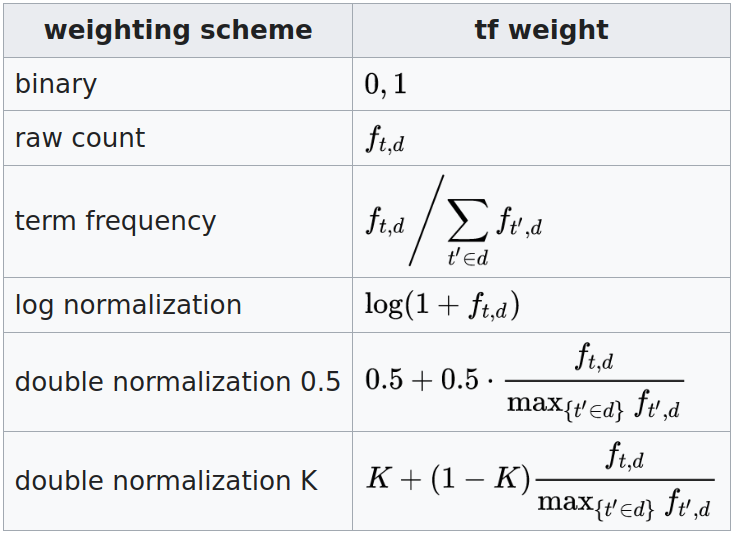
\includegraphics[width=13cm, angle=0]{Figures/VSM/variant-tf.png}}
	\end{center}
	\caption{Variant du TF \citep{sarch-engine-vsm}}
	\label{fig:variant-tf}
\end{figure}

\begin{figure}[htbp]
	\begin{center}
		\fbox{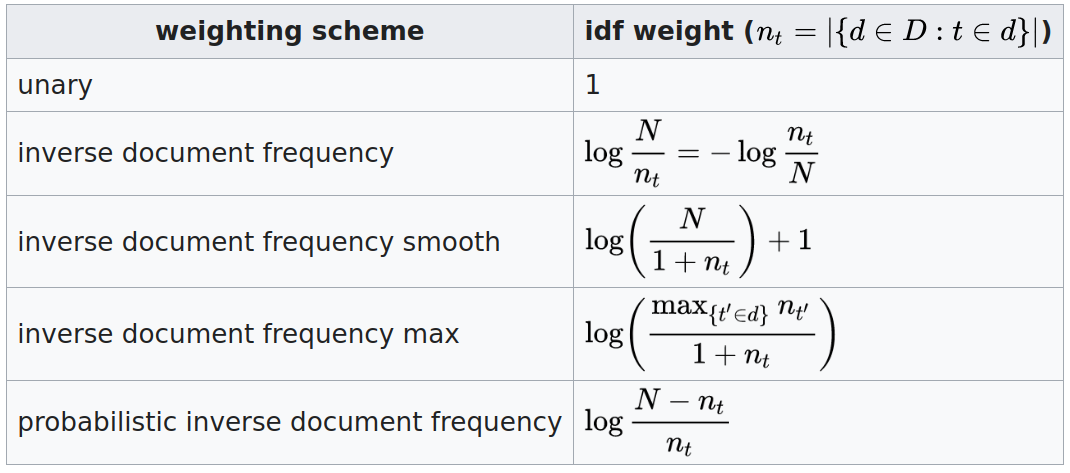
\includegraphics[width=15cm, angle=0]{Figures/VSM/variant-idf.png}}
	\end{center}
	\caption{Variant de l'IDF \citep{sarch-engine-vsm}}
	\label{fig:variant-idf}
\end{figure}

\begin{figure}[htbp]
	\begin{center}
		\fbox{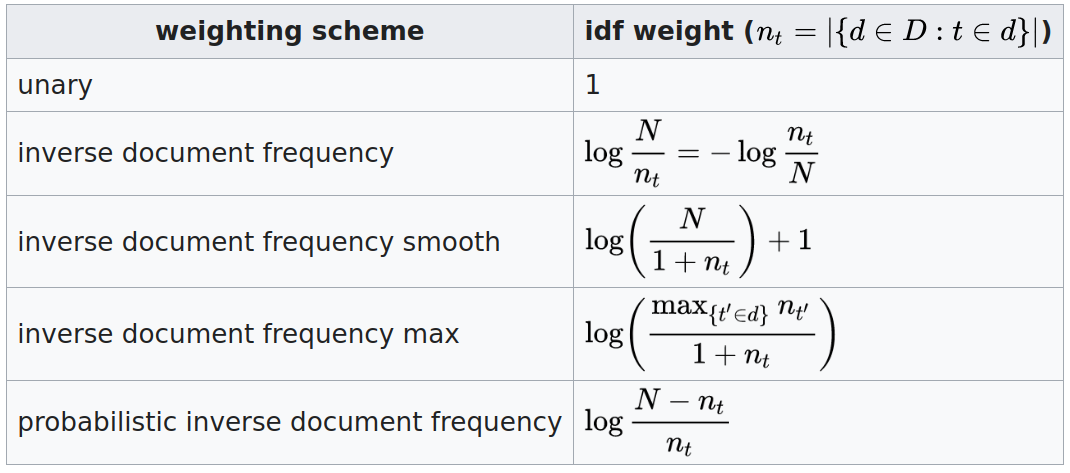
\includegraphics[width=15cm, angle=0]{Figures/VSM/variant-idf.png}}
	\end{center}
	\caption{Variant du TF-IDF \citep{sarch-engine-vsm}}
	\label{fig:variant-tf-idf}
\end{figure}

\section{Document inversé}
Le document inversé ou fichier inversé (Inverted index) permet de representer les documents ainsi que l'ensemble des termes dans la base de données, ainsi que ses poids calculés par ce méthode de pondération.

\section{Avantages}
Le modèle vectoriel a certains avantages: Facile a mettre en œuvre, possibilité d'avoir un appariement approximatif avec un degré de pertinence (L'utilisateur reçoit des documents qui pourrait lui intéressé), possibilité d'organiser les résultats suivant leur pertinence (L'utilisateur passe moins de temps a filtrer les résultats puisqu'ils sont déjà ordonné), ainsi ce modèle peut définir une limité pour la mesure de similarité et de n'afficher que les documents qui sont en dessus de cette limite pour éliminer les résultats le moins pertinent. Ce modèle est populaire, et plus utilisé par les moteurs de recherche actuel. \citep*{approche-semantique, modern-ir, soulier2014:def-evaluation-modele}

\section{Inconvénients}
Mais ce modèle a un inconvénients, qui est l’indépendance des termes d'indexation ce qui implique que la notion de sémantique du document est perdue. Mais ce problème a été solutionné par la mise place de regroupement des termes qui ont la même sens, on appelle N-grammes. Ou bien une autre approche est d'utiliser le modèle d’indexation sémantique latente (Latent Semantic Index).

\section{Conclusion}
Conclusion sur le VSM